\subsection{DAW, EQing \& Mischpulte}

\subsubsection{Mischpulte}

Ein Mischpult in der Tontechnik ist ein Gerät um verschieden Quellen \\(Mikrofone, Instrumente, ...) auf zwei (oder mehr) Ausganssummen oder -busse ( Untersummen mehrerer Signale) zusammenzufügen. 
Um einen guten Überblick zu erhalten empfehle ich noch mal \href{https://www.tontechnik-seminar.de/mischpult/mischpult-beispiel/}{hier} rein zu schauen.\\~\\

Ein Mischpult dient zur Bearbeitung von:\vspace{-3mm}
\begin{itemize}
    \item Klang
    \item Dynamik (Umfang der Lautstärke)
        \begin{itemize}
            \item generische Popmusik $\rightarrow$ sehr geringe Dynamik (\href{https://open.spotify.com/intl-de/track/6wgmzw64fvWGVNfDRbOHFh?si=d58caac6be5c46d1}{Spotify}~\href{https://youtu.be/w6LCfdzK92I?si=DPN0Gv5c4ZKfD83w}{YouTube})~
            \item klassische Musik $\rightarrow$ sehr große Dynamik (\href{https://open.spotify.com/intl-de/track/3gFQOMoUwlR6aUZj81gCzu?si=92ac7cfb89344e18}{Spotify}~\href{https://youtu.be/fawhjImDdJA?si=hyUGufzkj1buqda6}{YouTube})
        \end{itemize}
    \item Räumlichkeit
    \item Lautstärken (oder Verhältnisse)
\end{itemize}


\subsubsection{EQing}

\paragraph{Grundsätzlich Ansätze vom Filtern}~\\
\begin{itemize}
    \item Additives filtern\\
    Frequenzbereiche anheben -> Signal nach vorn holen, partiell hörbar machen, Griffigkeit, aber auch Aggressivität im Klang, Phasenprobleme werden betont.
    \item Subtraktives filtern\\
    Frequenzbereich absenken -> schlecht klingendes Absenken, Klarheit schaffen, Durchsichtigkeit, Phasenprobleme verstehen.
\end{itemize}

\newpage
\paragraph{Klanggestaltung (Equalizer und Filtersektion}
\begin{itemize}
    \item Shelving Filter\\
        Einsatzfrequenz $f$\\
        Gain (Anhebung / Absenkung in dB)
        \begin{figure}[h]
            \centering
            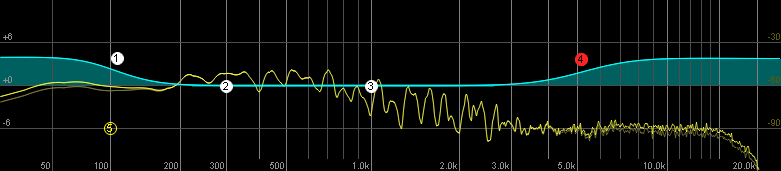
\includegraphics[width=0.5\linewidth]{Bilder/Medientechnik/Shelf.png}
            \caption{Caption}
            \label{fig:enter-label}
        \end{figure}

    \item Parametrischer EQ / Glockenfilter\\
        Frequenz $f$\\
        Gain in $dB$\\
        Güte (Breite) $Q$\\
        \begin{figure}[h]
            \centering
            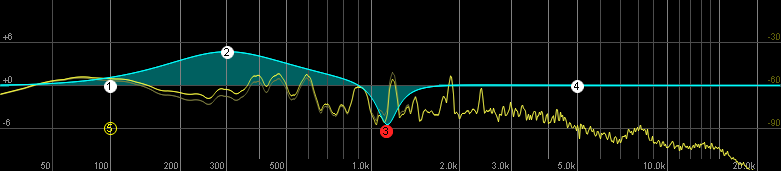
\includegraphics[width=0.5\linewidth]{Bilder/Medientechnik/Glockenfilter.png}
            \caption{Glockenfilter}
            \label{fig:enter-label}
        \end{figure}
    
    \item Low Cut und High Cut\\
        -3dB Einsatzfrequenz, Flankensteilheilt in dB/Oktave\\
\begin{figure}[h]
    \centering
    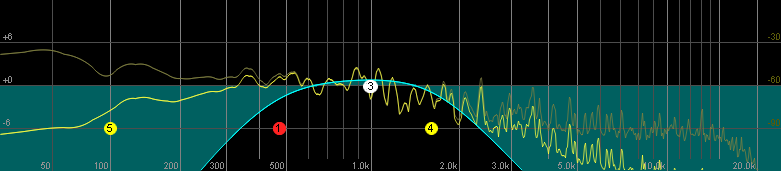
\includegraphics[width=0.5\linewidth]{Bilder/Medientechnik/LowHighpass.png}
    \caption{Lowcut und Highcut}
    \label{fig:Lowcut, Highcut}
\end{figure}
        Low Cut = Hochpass (hohe Frequenzen können passieren)\\
        High Cut = Tiefpass (tiefe Frequenzen können passieren)\\
\end{itemize}

\newpage

\paragraph{Kompressor}~
\begin{figure}[h]
    \centering
    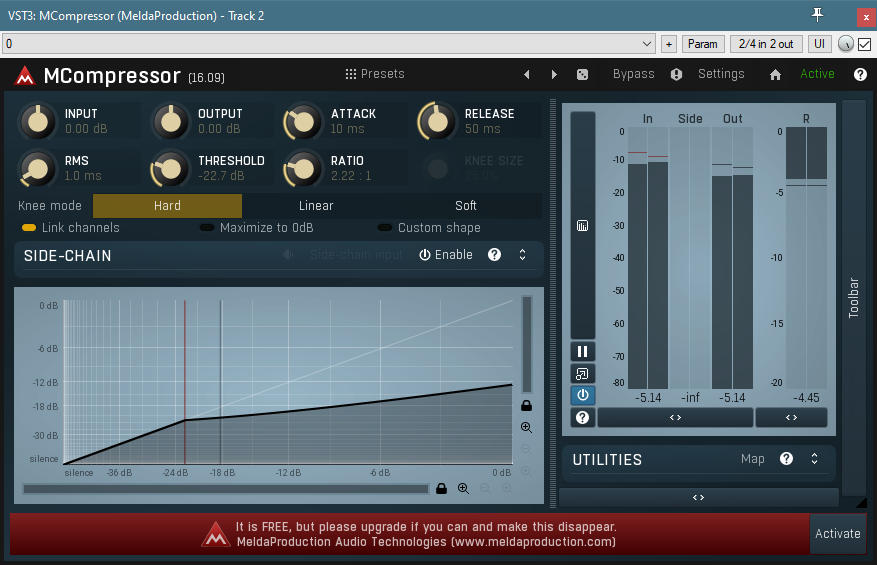
\includegraphics[width=0.5\linewidth]{Bilder/Medientechnik/Kompressor.png}
    \caption{Kopressor}
    \label{fig:enter-label}
\end{figure}

Ein Kompressor reduziert laute Töne über einem bestimmten Schwellenwerte.

\begin{figure}[h]
    \centering
    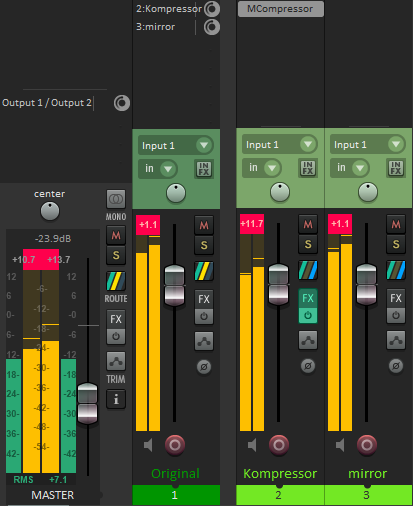
\includegraphics[width=0.5\linewidth]{Bilder/Medientechnik/Dualband-kompressor.png}
    \caption{Dualbandkompressor}
    \label{fig:Dualband-Kompressor}
\end{figure}
Dieser Funktioniert indem ein Ausgangssignal (hier Original) wird auf 2 Kanäle gesendet, wobei ein Kanal ein Kompressor drauf hat und der andere  einfach den normalen Ton.  Diese werden dann im Endmix zusammengeführt, was dazu führt das die Lauten Töne leiser sind und die leisen lauter (weil 2 Spuren aufaddiert werden).